%%%%%%%%%%%%%%%%%%%%%%%%%%%%%%%%%%%%%%%%%
% Beamer Presentation
% LaTeX Template
% Version 1.0 (10/11/12)
%
% This template has been downloaded from:
% http://www.LaTeXTemplates.com
%
% License:
% CC BY-NC-SA 3.0 (http://creativecommons.org/licenses/by-nc-sa/3.0/)
%
%%%%%%%%%%%%%%%%%%%%%%%%%%%%%%%%%%%%%%%%%

%----------------------------------------------------------------------------------------
%	PACKAGES AND THEMES
%----------------------------------------------------------------------------------------

\documentclass[aspectratio=169]{beamer}
%\documentclass{beamer}

\mode<presentation> {

% The Beamer class comes with a number of default slide themes
% which change the colors and layouts of slides. Below this is a list
% of all the themes, uncomment each in turn to see what they look like.

%\usetheme{default}
%\usetheme{AnnArbor}
%\usetheme{Antibes}
%\usetheme{Bergen}
%\usetheme{Berkeley}
%\usetheme{Berlin}
%\usetheme{Boadilla}
%\usetheme{CambridgeUS}
%\usetheme{Copenhagen}
%\usetheme{Darmstadt}
%\usetheme{Dresden}
%\usetheme{Frankfurt}
%\usetheme{Goettingen}
%\usetheme{Hannover}
%\usetheme{Ilmenau}
%\usetheme{JuanLesPins}
%\usetheme{Luebeck}
\usetheme{Madrid}
%\usetheme{Malmoe}
%\usetheme{Marburg}
%\usetheme{Montpellier}
%\usetheme{PaloAlto}
%\usetheme{Pittsburgh}
%\usetheme{Rochester}
%\usetheme{Singapore}
%\usetheme{Szeged}
%\usetheme{Warsaw}

% As well as themes, the Beamer class has a number of color themes
% for any slide theme. Uncomment each of these in turn to see how it
% changes the colors of your current slide theme.

%\usecolortheme{albatross}
%\usecolortheme{beaver}
%\usecolortheme{beetle}
%\usecolortheme{crane}
%\usecolortheme{dolphin}
%\usecolortheme{dove}
%\usecolortheme{fly}
%\usecolortheme{lily}
%\usecolortheme{orchid}
%\usecolortheme{rose}
%\usecolortheme{seagull}
%\usecolortheme{seahorse}
%\usecolortheme{whale}
%\usecolortheme{wolverine}

%\setbeamertemplate{footline} % To remove the footer line in all slides uncomment this line
%\setbeamertemplate{footline}[page number] % To replace the footer line in all slides with a simple slide count uncomment this line

%\setbeamertemplate{navigation symbols}{} % To remove the navigation symbols from the bottom of all slides uncomment this line
}

\usepackage{graphicx} % Allows including images
\usepackage{booktabs} % Allows the use of \toprule, \midrule and \bottomrule in tables
%\RequirePackage{beamerthemeoracle}

%----------------------------------------------------------------------------------------
%	TITLE PAGE
%----------------------------------------------------------------------------------------

\title[Xen Overview]{Xen Virtualization Overview} % The short title appears at the bottom of every slide, the full title is only on the title page

\author{Dongli Zhang} % Your name
\institute[Oracle] % Your institution as it will appear on the bottom of every slide, may be shorthand to save space
{
Oracle Asia Research and Development Centers (Beijing) \\ % Your institution for the title page
\medskip
\textit{dongli.zhang@oracle.com} % Your email address
}
\date{\today} % Date, can be changed to a custom date

\begin{document}

%------------------------------------------------

\section{Title}
\begin{frame}
\titlepage % Print the title page as the first slide
\end{frame}

%------------------------------------------------

\section{What is virtualization}
\begin{frame}
\frametitle{What is virtualization}
A virtual machine is taken to be an efficient, isolated duplicate of the real machine. (Gerald J.Popek and Rebert P. Goldberg, 1974) \pause
\begin{itemize}
\item \textbf{efficient}: capable of producing desired results without wasting materials, time, or \textcolor<3->{red}{energy}\pause \pause
\item \textbf{isolated}: separate from others; happening in different places and at different times
\begin{figure}
%\begin{subfigure}{.5\textwidth}
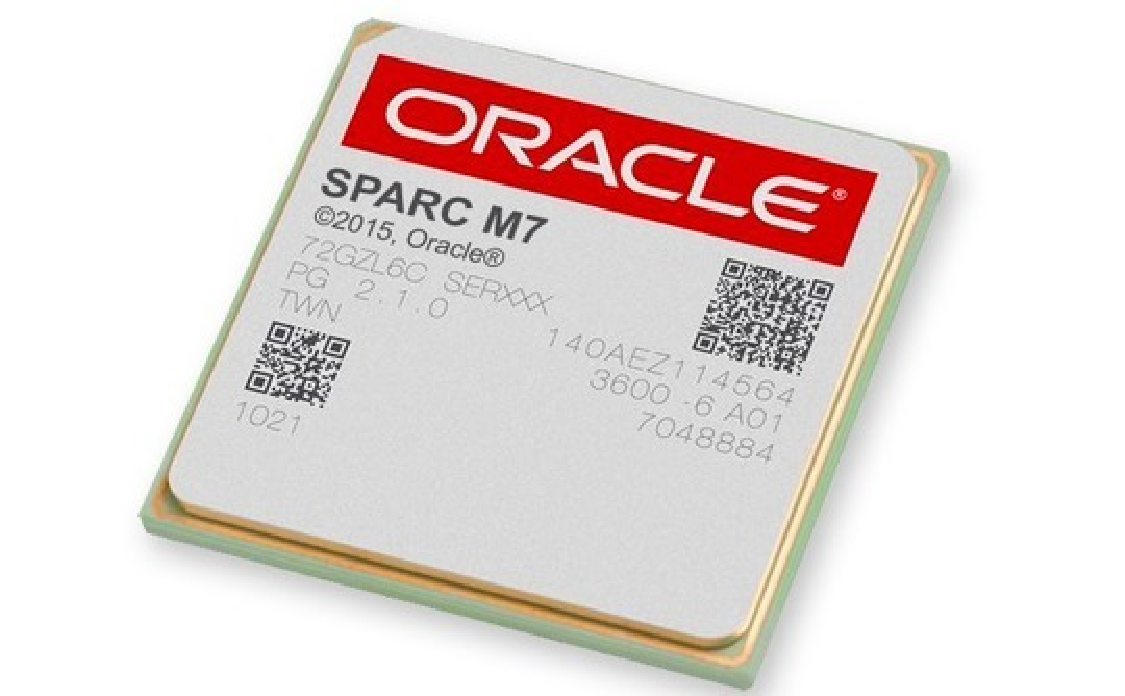
\includegraphics[width=0.3\linewidth]{figures/sparc.pdf}
%\end{subfigure}
\end{figure}
\end{itemize}
\end{frame}

%------------------------------------------------

\section{Trap and Emulate}
\begin{frame}
\frametitle{Trap and Emulate}
\begin{figure}
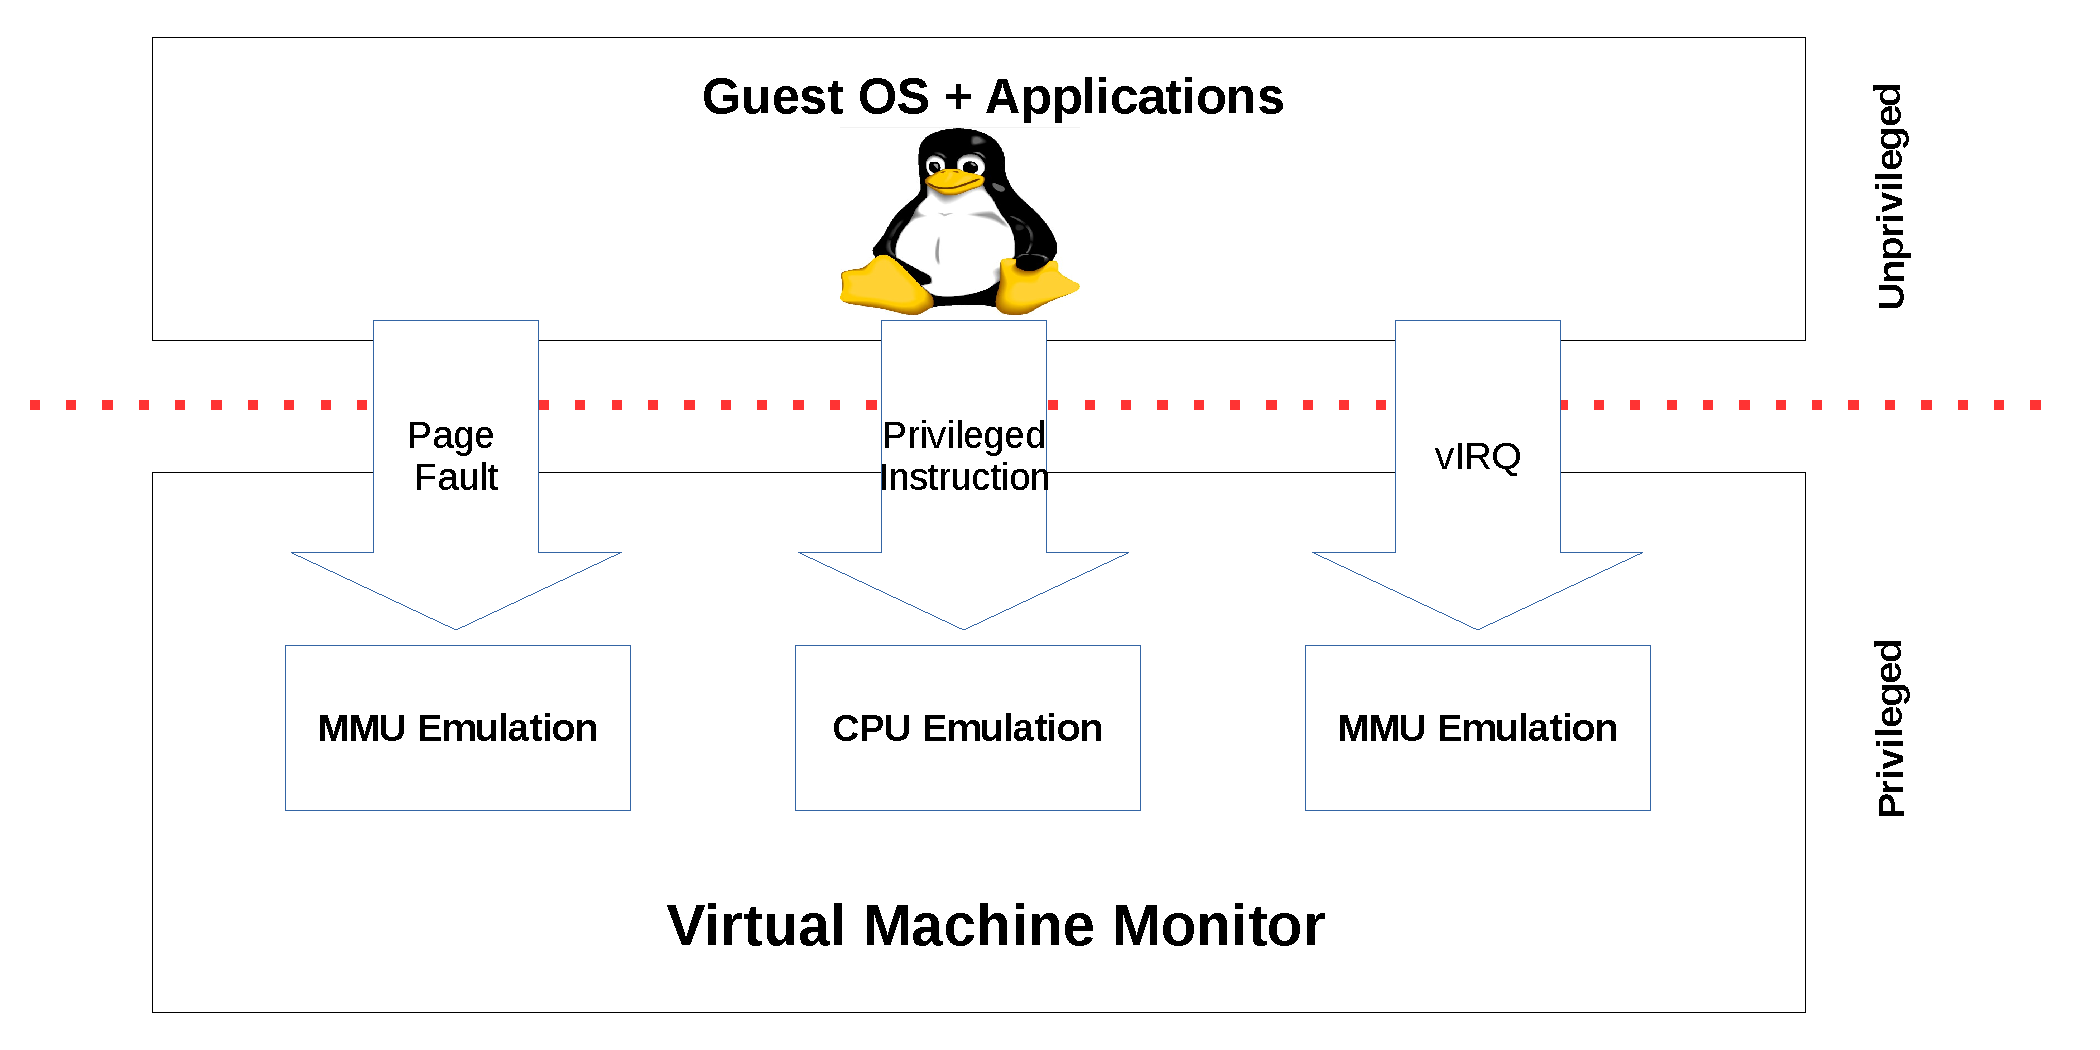
\includegraphics[width=1.0\linewidth]{figures/trapemu.pdf}
\end{figure}
\end{frame}

%------------------------------------------------

\section{Hardware Virtualization (Intel VT)}
\begin{frame}
\frametitle{Hardware Virtualization (Intel VT)}
\begin{figure}
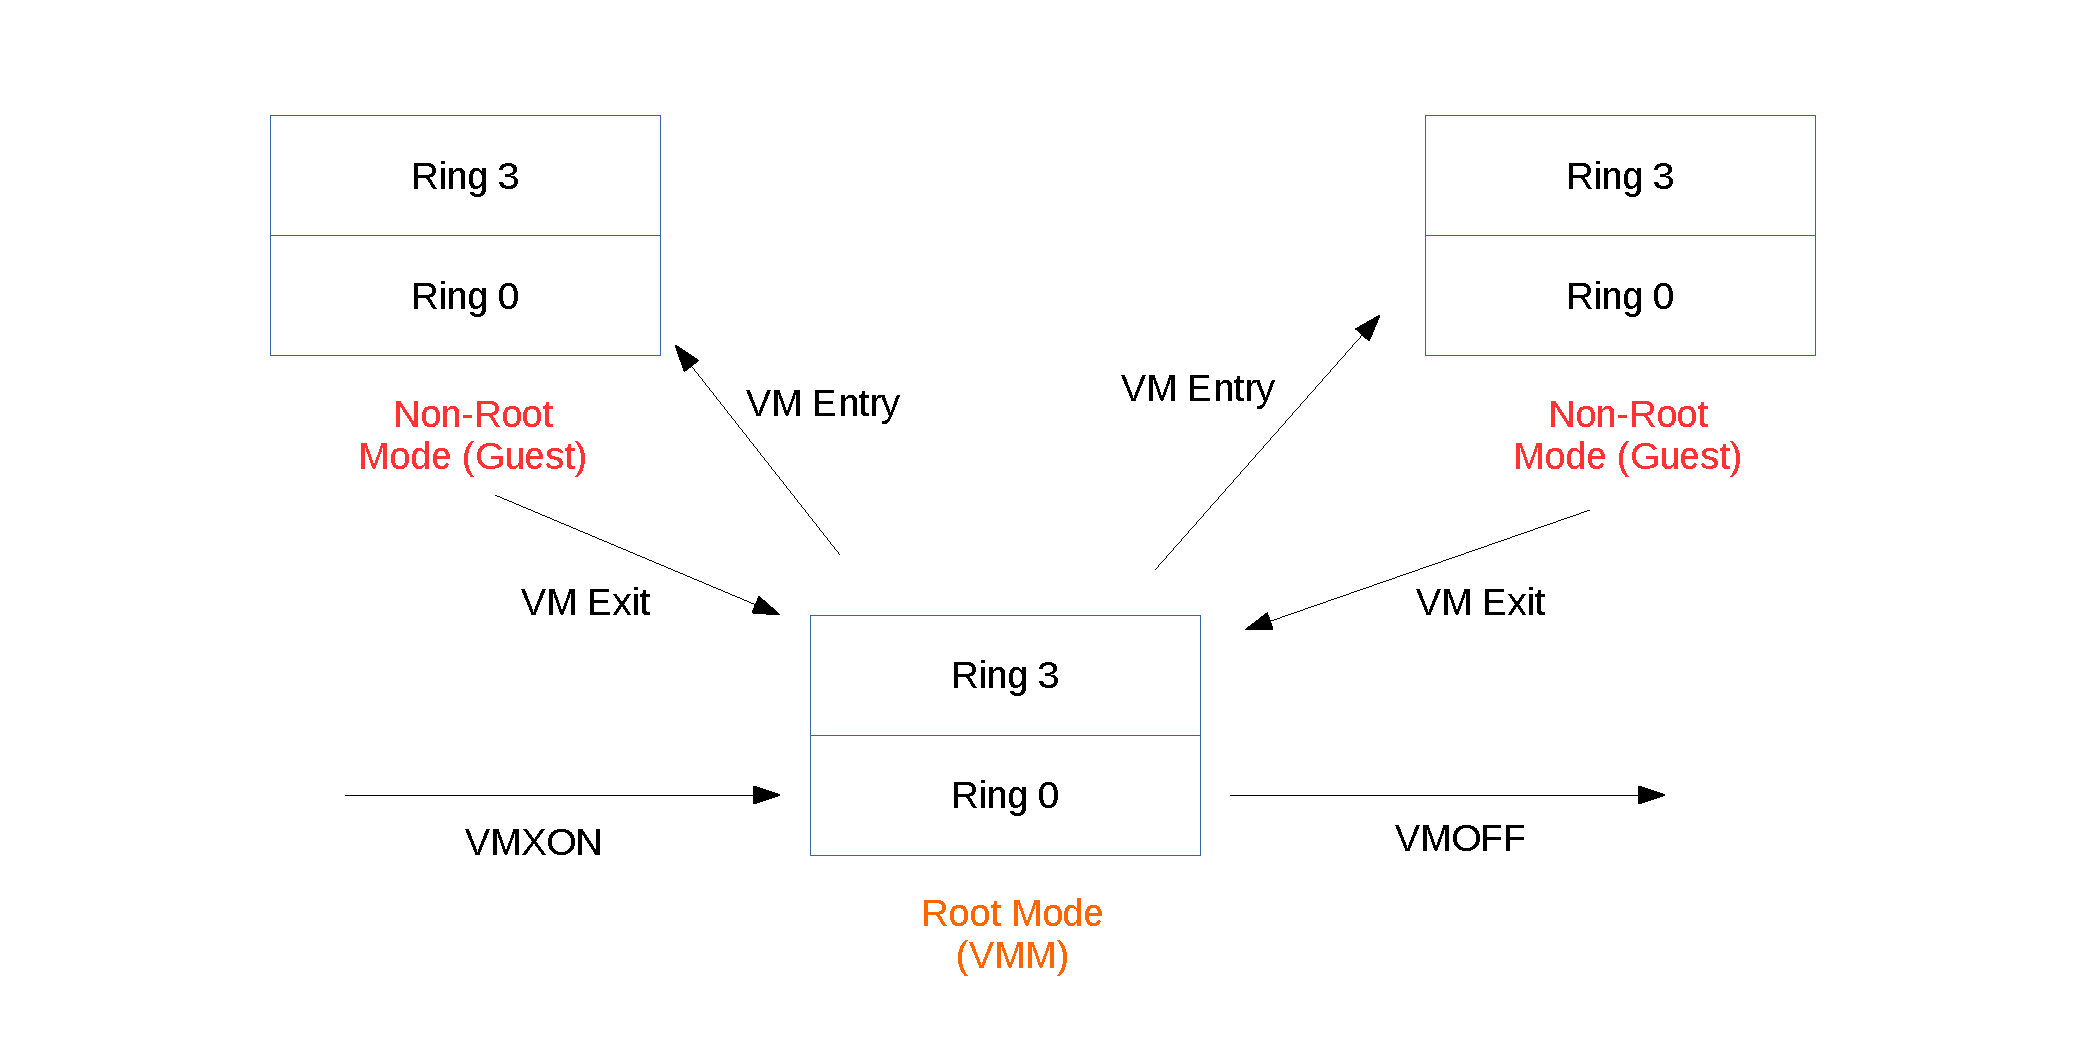
\includegraphics[width=1.0\linewidth]{figures/vmx.pdf}
\end{figure}
\end{frame}

%------------------------------------------------

\section{KVM (Kernel-based Virtual Machine)}
\begin{frame}
\frametitle{KVM (Kernel-based Virtual Machine)}
\begin{columns}[c]
\column{.5\textwidth}
\begin{center}
\begin{itemize}
\item CPU hardware virtualization extensions (Intel VT or AMD-V)
\item Loadable kernel module (kvm.ko, kvm-intel.ko/kvm-amd.ko)
\item QEMU as userspace emulator
\end{itemize}
\end{center}
\column{.5\textwidth}
\begin{center}
\begin{figure}
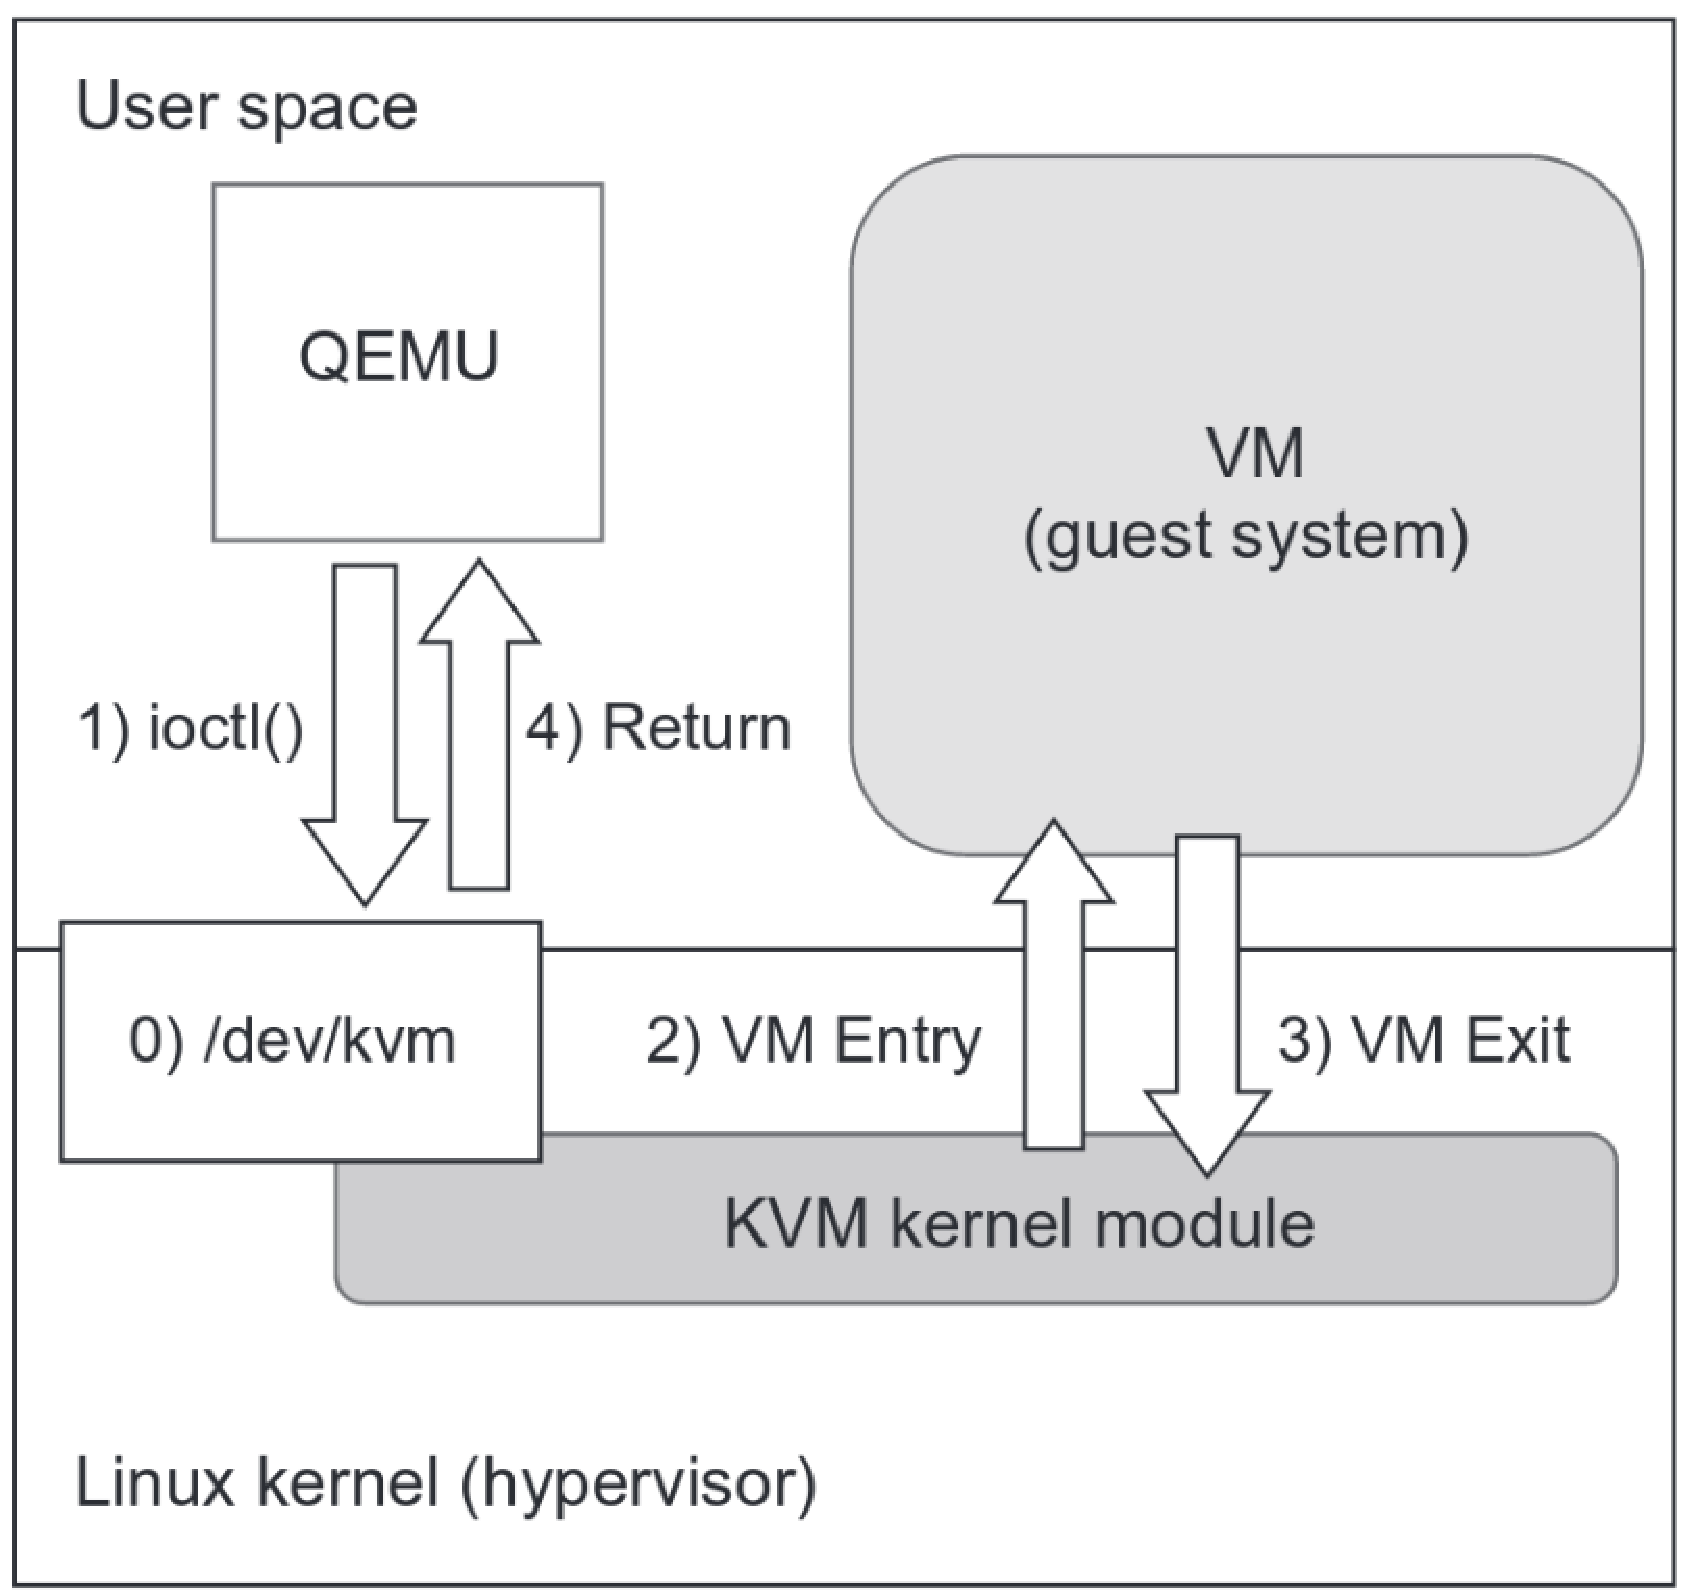
\includegraphics[width=1.0\linewidth]{figures/kvm.pdf}
\end{figure}
\end{center}
\end{columns}
\end{frame}

%------------------------------------------------

\section{State of the Art Virtualization}
\begin{frame}
\frametitle{State of the Art Virtualization}
\begin{itemize}
\item Instruction Emulator (QEMU, Bochs) \pause
\item Paravirtualization (Xen) \pause
\item Hardware-assisted Virtualization (KVM, Xen, VMware) \pause
\item OS-level Virtualization (Linux Container) \pause
\item Programming Language Virtualization (Java, .NET CLR) \pause
\item Library Virtualization (Wine, Cygwin)
\end{itemize}
\end{frame}

%------------------------------------------------

\section {What is Xen}
\begin{frame}
\frametitle{What is Xen}
\begin{block}{Wikipedia}
Xen Project is a hypervisor using a microkernel design, providing services that allow multiple computer operating systems to execute on the same computer hardware concurrently.
\end{block} \pause
\begin{block}{SOSP 2003: Xen and the Art of Virtualization}
This paper presents Xen, an x86 virtual machine monitor which allows multiple commodity operating systems to share conventional hardware in a safe and resource managed fashion, but without sacrificing either performance or functionality. \pause
\end{block}
\begin{block}{Basic Idea of Paravirtualization}
Actively tell the hypervisor what the guest is going to do
\end{block}
\end{frame}

%------------------------------------------------

\section{Xen Framework}
\begin{frame}
\frametitle{Xen Framework}
\begin{figure}
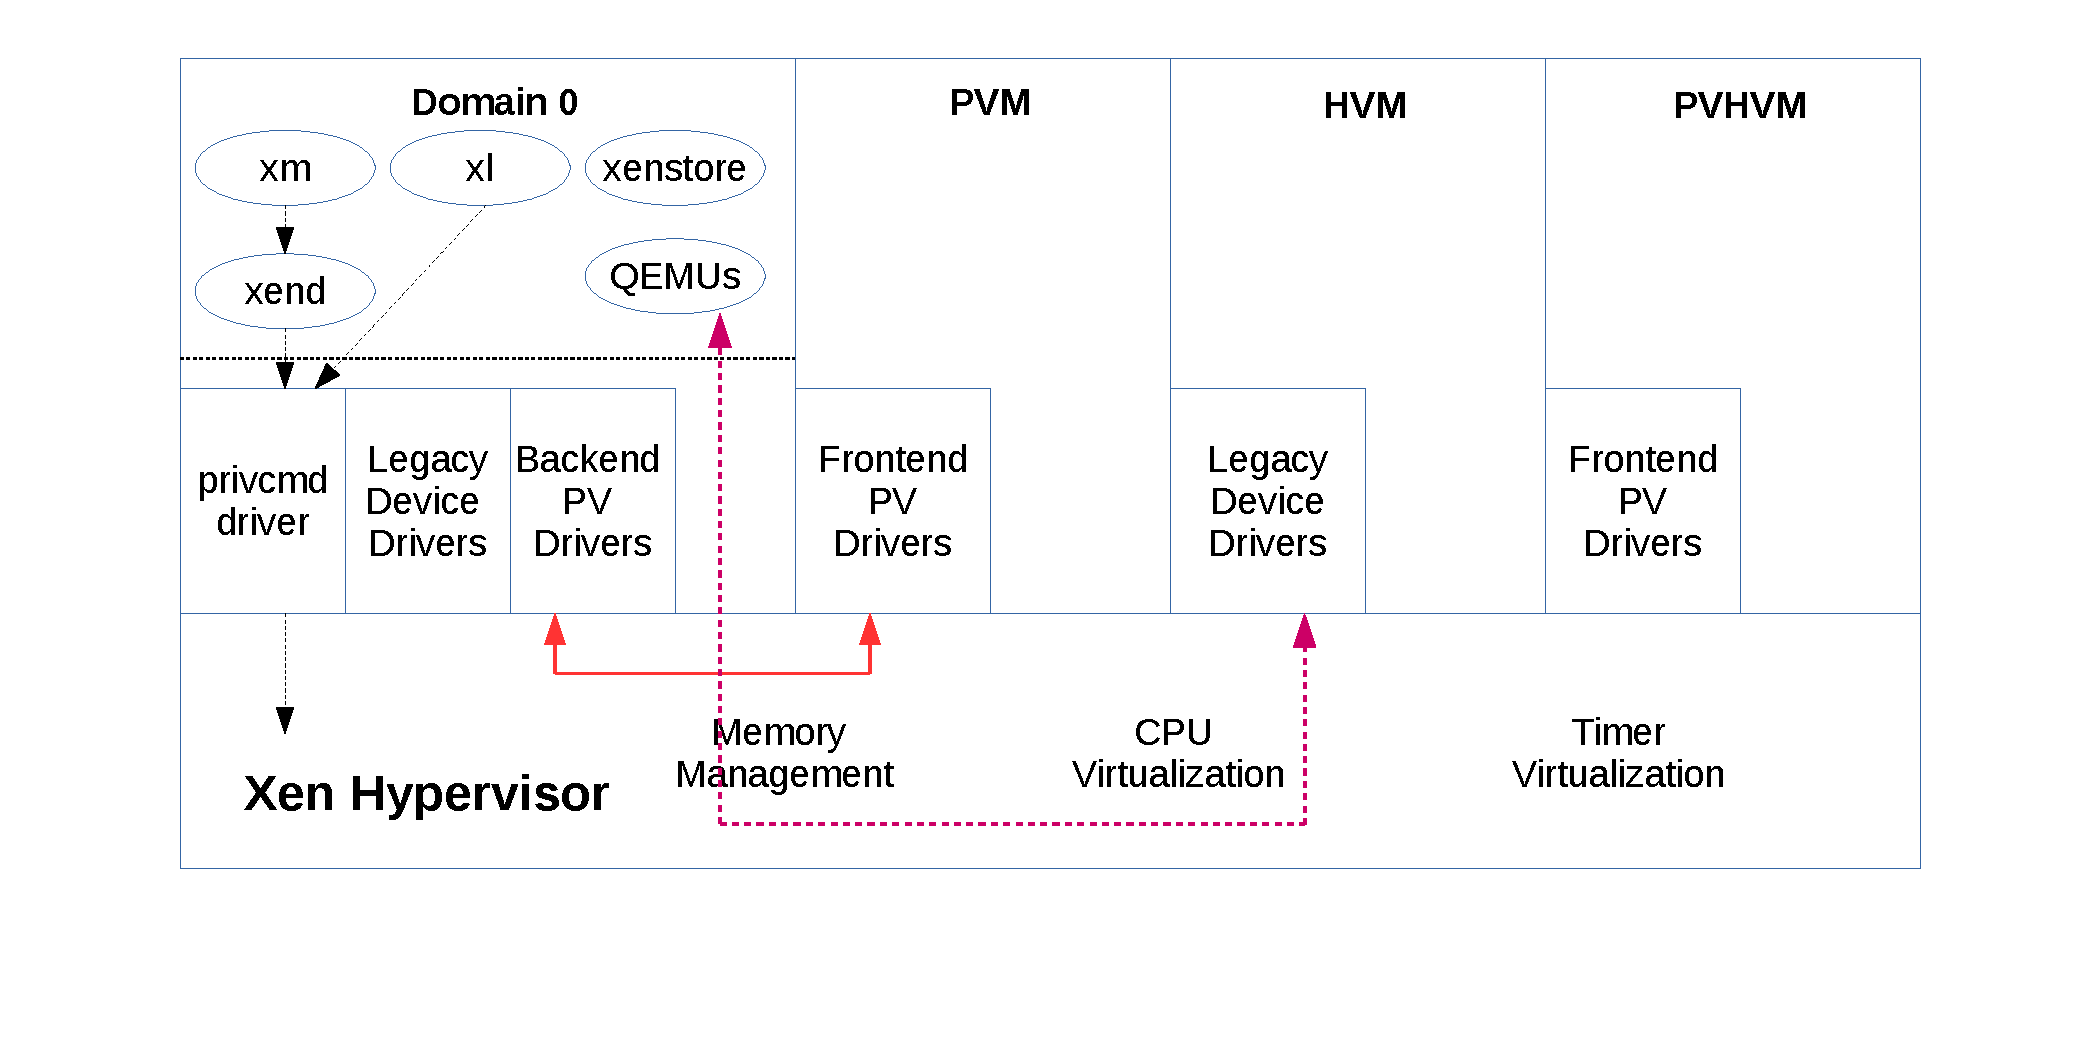
\includegraphics[width=1.0\linewidth]{figures/xen.pdf}
\end{figure}
\end{frame}

%------------------------------------------------

\begin{frame}
\frametitle{PV, HVM or PVHVM}
\begin{figure}
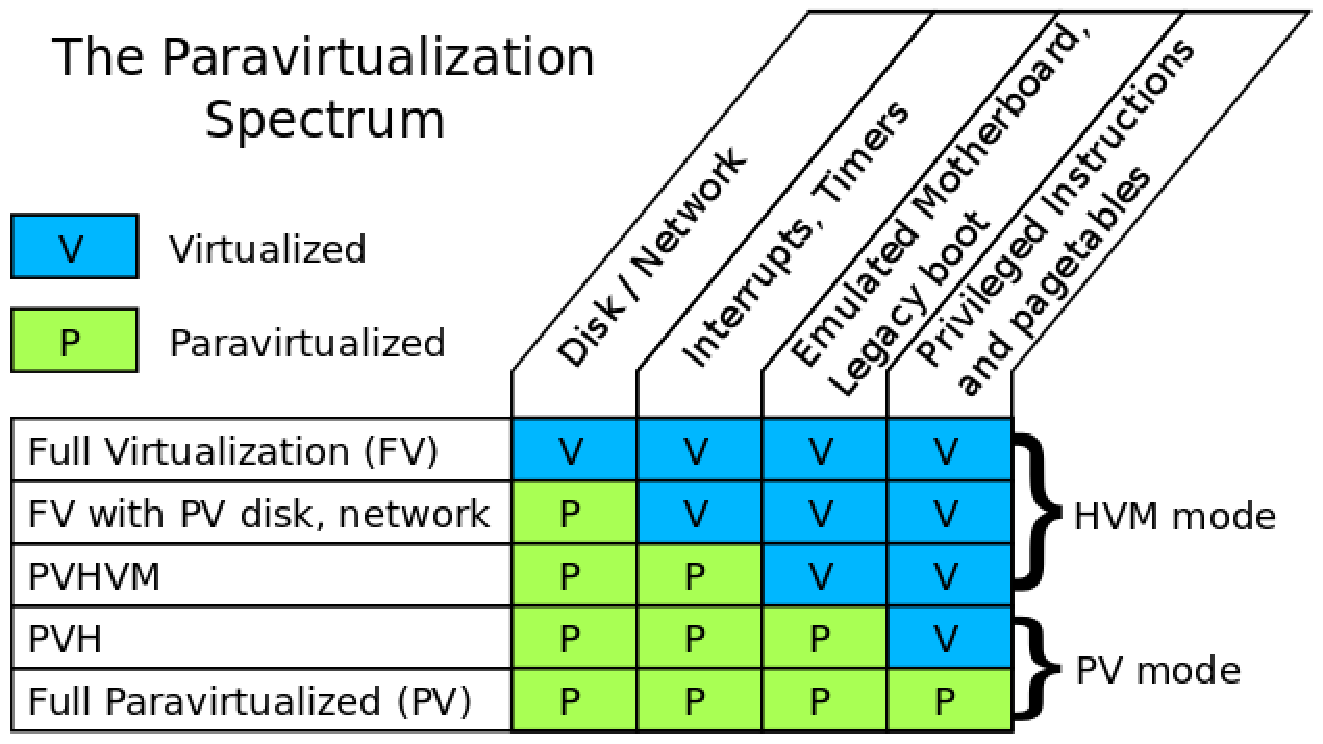
\includegraphics[width=0.8\linewidth]{figures/spectrum.pdf}
\end{figure}
\end{frame}

%------------------------------------------------

\begin{frame}
\frametitle{Xen CPU Virtualization}
\end{frame}

%------------------------------------------------

\begin{frame}
\frametitle{Xen Interrupt Virtualization}
\end{frame}

%------------------------------------------------

\begin{frame}
\frametitle{Xen Timer Virtualization}
\end{frame}

%------------------------------------------------

\begin{frame}
\frametitle{Xen Memory Virtualization}
\end{frame}

%------------------------------------------------

\begin{frame}
\frametitle{Xen Device Virtualization}
\begin{itemize}
\item HVM emulated legacy device (QEMU) \pause
\item \textbf<5->{\textcolor<5->{red}{Paravirtual (PV) drivers}} \pause
\item Device Passthrough (vt-d) \pause
\item Virtual Function (vt-d) \pause
\end{itemize}
\end{frame}

%------------------------------------------------

\section{PV driver vs. PCI driver}
\begin{frame}
\frametitle{PV driver vs. PCI driver}
\begin{table}
\small
\begin{tabular}{l l l}
\toprule
& \textbf{PCI driver} & \textbf{PV driver}\\
\midrule
device abstraction & pci\_device, pci\_driver & xenbus\_device, xenbus\_driver \\
device discovery & PCI Tree & Xenstore \\
device configuration & PCI Config Space (IO/MMIO) & Xenstore \\
data flow & DMA Ring Buffer & Memory Ring Buffer \\
shared memory & IOMMU & Grant Table \\
interrupt & IOAPIC, MSI, MSI-X & Event Channel \\
\bottomrule
\end{tabular}
\end{table}
\end{frame}

%------------------------------------------------

\section{Xenstore/Xenbus}
\begin{frame}
\frametitle{Xenstore/Xenbus}
\begin{figure}
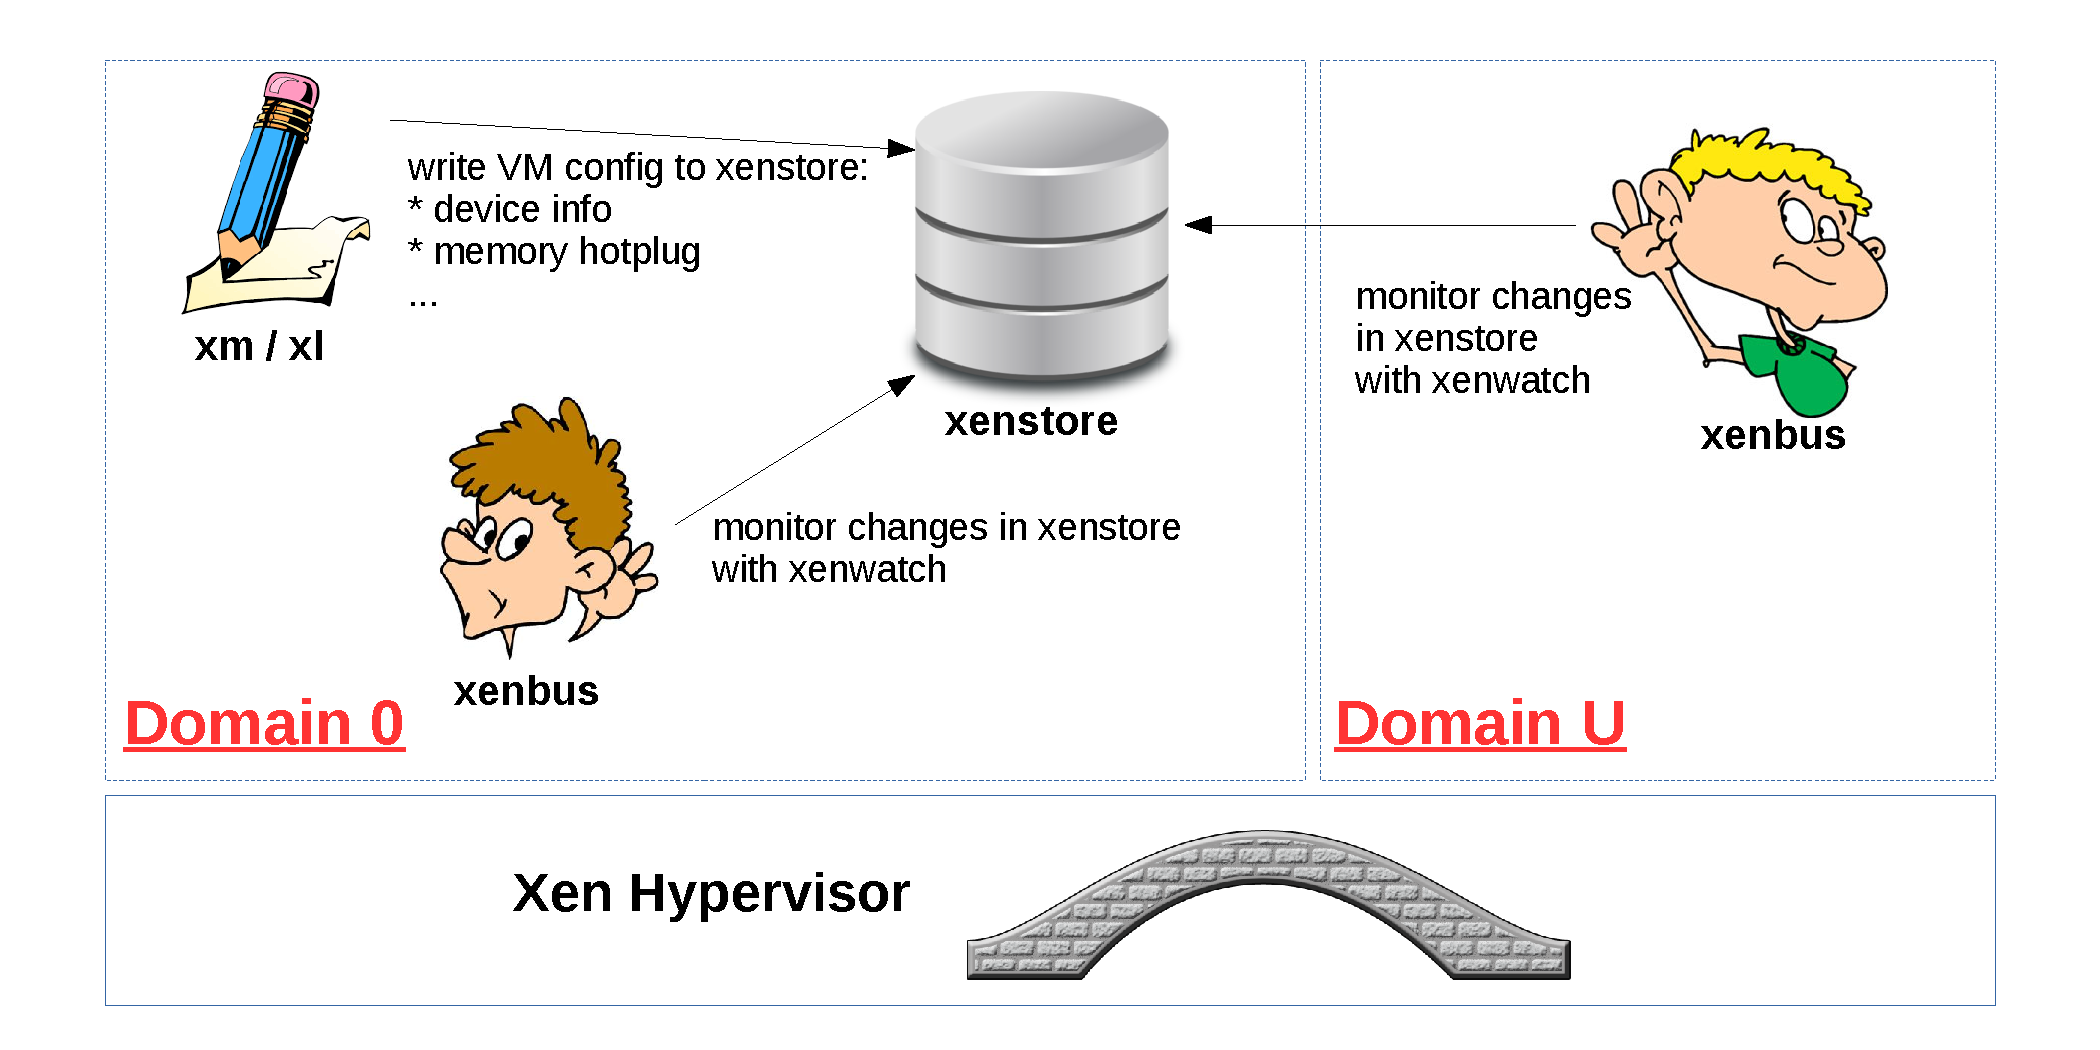
\includegraphics[width=1.0\linewidth]{figures/xenstore.pdf}
\end{figure}
\end{frame}

%------------------------------------------------

\section{Grant Table}
\begin{frame}
\frametitle{Grant Table}
\begin{figure}
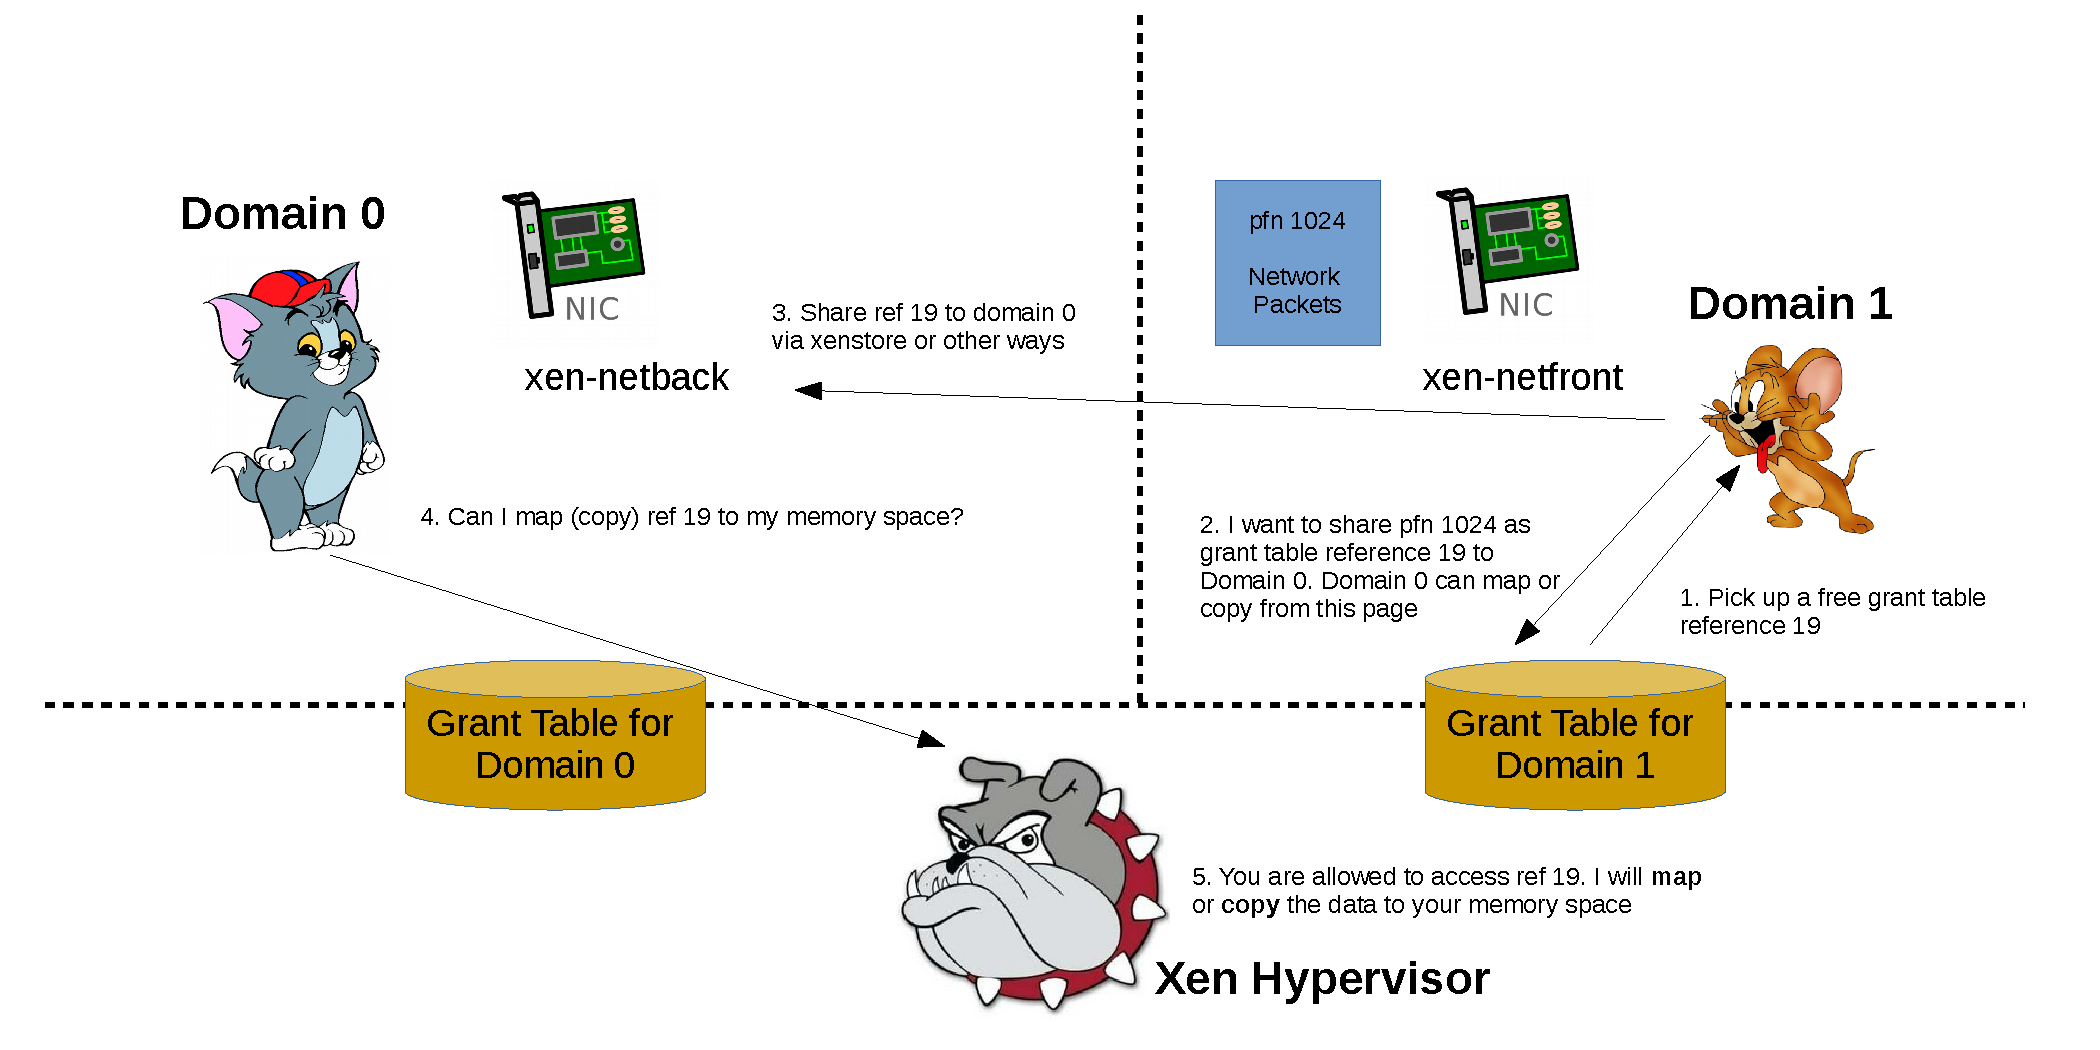
\includegraphics[width=1.0\linewidth]{figures/grant.pdf}
\end{figure}
\end{frame}

%------------------------------------------------

\section{I/O Ring Buffer}
\begin{frame}
\frametitle{I/O Ring Buffer}
\begin{columns}[c]
\column{.6\textwidth}
\begin{center}
\begin{itemize}
\item Usually put grant ref (not data) in ring
\item Grant ref of ring pages are shared via xenstore
\item Usually one ring buffer for each device queue
\item One or more pages for each ring
\item Producer and Consumer (barrier)
\end{itemize}
\end{center}
\column{.4\textwidth}
\begin{center}
\begin{figure}
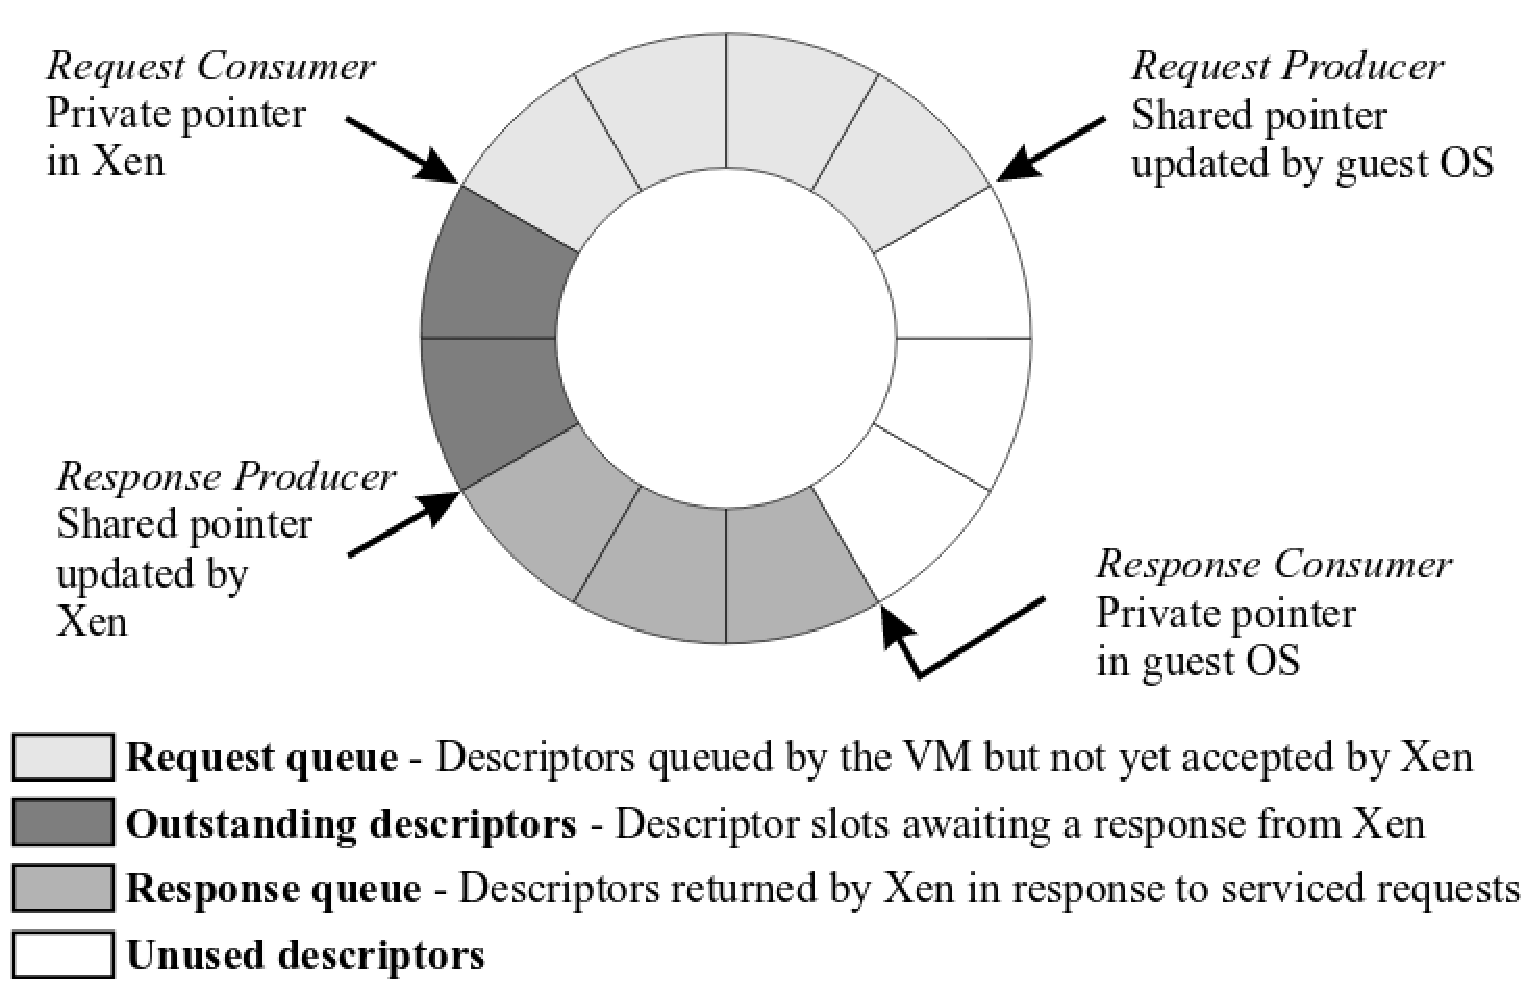
\includegraphics[width=1.0\linewidth]{figures/ring.pdf}
\end{figure}
\end{center}
\end{columns}
\end{frame}

%------------------------------------------------

\section{Event Channel}
\begin{frame}
\frametitle{Event Channel}
\begin{block}{Registration}
\begin{itemize}
\item PVM registers event channel handler to Xen via 

register\_callback(CALLBACKTYPE\_event, xen\_hypervisor\_callback)

\item PVHVM sets HYPERVISOR\_CALLBACK\_VECTOR via

HYPERVISOR\_hvm\_op(HVMOP\_set\_param, \&a)
\end{itemize}
\end{block}
\begin{block}{Types}
\begin{itemize}
\item Interdomain Event
\item Virtual IRQ Event
\item Physical IRQ Event
\item IPI Event
\end{itemize}
\end{block}
\end{frame}

%------------------------------------------------

\section{PV driver from scratch}
\begin{frame}
\frametitle{PV driver from scratch}
\end{frame}

%------------------------------------------------

\section{Take-Home Message}
\begin{frame}
\frametitle{Take-Home Message}
\begin{itemize}
\item What is virtualization
\item Paravirtualization and Hardware-assisted Virtualization
\item Xen vs. KVM
\item Grant Table, Event Channel, Paravirtual Drivers
\end{itemize}
\end{frame}

%\begin{frame}
%\Huge{\centerline{The End}}
%\end{frame}

%----------------------------------------------------------------------------------------

\end{document} 
